\documentclass[10pt]{article}
\usepackage[english]{babel}
\usepackage{../../../../lib/tex/naproche}
\usepackage{amssymb}
\usepackage{mathtools} % for \coloneq

\usepackage{stex-highlighting}
\providebool{emph} % "\newbool{emph}" does not work...
\setbool{emph}{false}
\colorlet{emphcolor}{violet}
\let\oldemph\emph
\renewcommand\emph[1]{\setbool{emph}{true}\ifbool{forthel}{\textcolor{emphcolor}{\itshape#1}}{\oldemph{#1}}\setbool{emph}{false}}
\renewcommand{\varemph}[1]{\ifbool{emph}{\textcolor{emphcolor}{#1}}{\textcolor{black}{#1}}}

\usepackage[right=6cm,left=3cm,bottom=3cm,marginparwidth=5cm]{geometry}

\usepackage{fancyhdr}
\renewcommand{\sectionmark}[1]{\markboth{#1}{}} 
\def\libarchive{}
\pagestyle{fancy}
\fancyhead[L]{\libarchive}
\fancyhead[C]{\nouppercase\leftmark}  % section title
\fancyhead[R]{\thepage}               % page number
\fancyfoot[C]{}                       % No page number in footer

\usepackage[nobottomtitles]{titlesec}
\titlespacing*{\section}{0pt}{30pt}{0pt}
\titlespacing*{\subsection}{0pt}{30pt}{0pt}
\titlespacing*{\subsubsection}{0pt}{30pt}{0pt}

\documentclass[12pt,oneside]{book}

\usepackage[foundations]{../../lib/tex/naproche}
\usepackage{../../lib/tex/libraries}
\usepackage{graphicx}
\usepackage{float}
\usepackage{caption}
\usepackage{footnote}

\makesavenoteenv{tabular} % Make footnotes work in tabular environments


\title{Foundations of Mathematics}
\author{Marcel Schütz}
\date{2022}

\begin{document}
  \maketitle

  \tableofcontents

  \begin{figure}[H]
    \centering
    \fbox{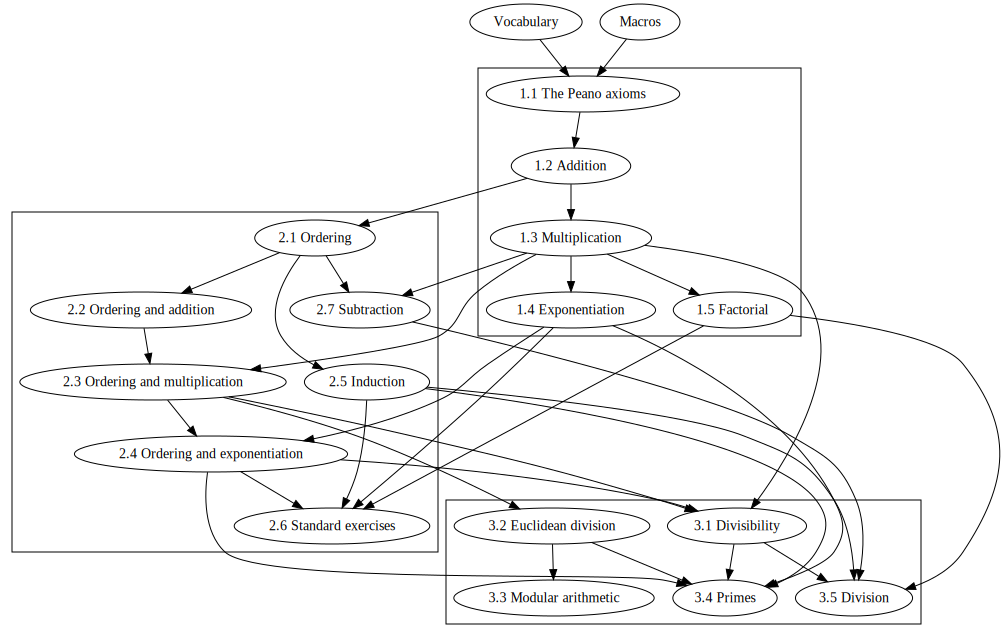
\includegraphics[width=0.9\linewidth]{./dependency-graph/graph.png}}
    \caption*{Interdependencies of the chapters}
  \end{figure}


  \section*{Introduction}

  This is a library providing a foundation of mathematics based on a
  Kelley-Morse like class theory with urelements.
  It introduces common operations on classes like unions or intersections
  (\cref{chapter:classes}) together with detailed proofs of their algebraic
  properties (\cref{chapter:computation-laws-for-classes}), the symmetric
  difference of two classes (\cref{chapter:symmetric-difference}) and the
  notions of ordered pairs and Cartesian products
  (\cref{chapter:pairs-and-products}) as well as proofs of the algebraic
  properties of the latter (\cref{chapter:computation-laws-for-products}).
  Moreover, it provides common operations on maps (\cref{chapter:maps}), various
  properties of images and preimages (\cref{chapter:image-and-preimage}) and the
  notions of injectivity, surjectivity, bijectivity
  (\cref{chapter:injections-surjections-bijections}) and invertibility of maps
  (\cref{chapter:invertible-maps}).
  The library provides an axiom system characterizing sets (\cref{chapter:sets})
  and, furthermore, it covers the notions of binary relations
  (\cref{chapter:binary-relations}), fixed-points of subset preserving maps
  (\cref{chapter:fixed-points}), including and equinumerosity
  (\cref{chapter:equinumerosity}).

  As two famous results it includes the Knaster-Tarski fixed point theorem
  (\cref{FOUNDATIONS_12_8420450166112256}) and the Cantor-Schröder-Bernstein
  theorem (\cref{FOUNDATIONS_13_1913663275401216}).

  \paragraph*{Usage.}
  At the very beginning of each chapter you can find the name of its source
  file, e.g. \path{foundations/sections/01_classes.ftl.tex} for
  \cref{chapter:classes}. This filename can be used to import the chapter via
  \Naproche's \texttt{readtex} instruction to another ForTheL text, e.g.:
  \begin{center}
    \verb`[readtex \path{foundations/sections/01_classes.ftl.tex}]`
  \end{center}

  \paragraph*{Checking times.}
  The checking times for each of the chapters may vary from computer to
  computer, but on mid-range hardware they are likely to be similar to those
  given in table below:

  \begin{center}
    \begin{tabular}{c|c|c}

      & \multicolumn{2}{c}{\textbf{Checking time}}
      \\
      \textbf{Chapter}
      & \textbf{without dependencies}     & \textbf{with dependencies}
      \\ \hline
      \ref{chapter:classes}
      & 00:04 min                         & 00:04 min
      \\
      \ref{chapter:computation-laws-for-classes}
      & 00:12 min                         & 00:16 min
      \\
      \ref{chapter:symmetric-difference}
      & 00:32 min                         & 00:48 min
      \\
      \ref{chapter:pairs-and-products}
      & 00:08 min                         & 00:12 min
      \\
      \ref{chapter:computation-laws-for-products}
      & 01:36 min                         & 01:56 min
      \\
      \ref{chapter:maps}
      & 01:13 min                         & 01:25 min
      \\
      \ref{chapter:image-and-preimage}
      & 01:28 min                         & 02:53 min
      \\
      \ref{chapter:injections-surjections-bijections}
      & 00:38 min                         & 02:03 min
      \\
      \ref{chapter:invertible-maps}
      & 02:20 min                         & 04:23 min
      \\
      \ref{chapter:sets}
      & 02:17 min                         & 06:40 min
      \\
      \ref{chapter:binary-relations}
      & 00:14 min                         & 06:54 min
      \\
      \ref{chapter:fixed-points}
      & 00:33 min                         & 07:13 min
      \\
      \ref{chapter:equinumerosity}
      & 01:48 min                         & 09:01 min
    \end{tabular}
  \end{center}


  \subfile{sections/01_classes.ftl.tex}
  \subfile{sections/02_computation-laws-for-classes.ftl.tex}
  \subfile{sections/03_symmetric-difference.ftl.tex}
  \subfile{sections/04_pairs-and-products.ftl.tex}
  \subfile{sections/05_computation-laws-for-products.ftl.tex}
  \subfile{sections/06_maps.ftl.tex}
  \subfile{sections/07_image-and-preimage.ftl.tex}
  \subfile{sections/08_injections-surjections-bijections.ftl.tex}
  \subfile{sections/09_invertible-maps.ftl.tex}
  \subfile{sections/10_sets.ftl.tex}
  \subfile{sections/11_binary-relations.ftl.tex}
  \subfile{sections/12_fixed-points.ftl.tex}
  \subfile{sections/13_equinumerosity.ftl.tex}
\end{document}

\documentclass[12pt,oneside]{book}

\usepackage[utf8]{inputenc}
\usepackage[english]{babel}

\usepackage{../meta-inf/lib/naproche-logo}
\usepackage{../meta-inf/lib/naproche}
\usepackage{../meta-inf/lib/libraries}
\usepackage{naproche}
\usepackage{naproche-libraries}
\renewcommand\libarchive{Preliminaries}
\usepackage{naproche}
\usepackage{naproche-libraries}
\renewcommand\libarchive{Preliminaries}

\usepackage{xr}
\externaldocument{../foundations/foundations}

\usepackage{graphicx}
\usepackage{float}
\usepackage{caption}
\usepackage[nobottomtitles]{titlesec}


\title{Set theory}
\author{Marcel Schütz}
\date{2022}

\begin{document}
  \maketitle

  \tableofcontents

  \paragraph*{}
  \begin{figure}[H]
    \centering
    \fbox{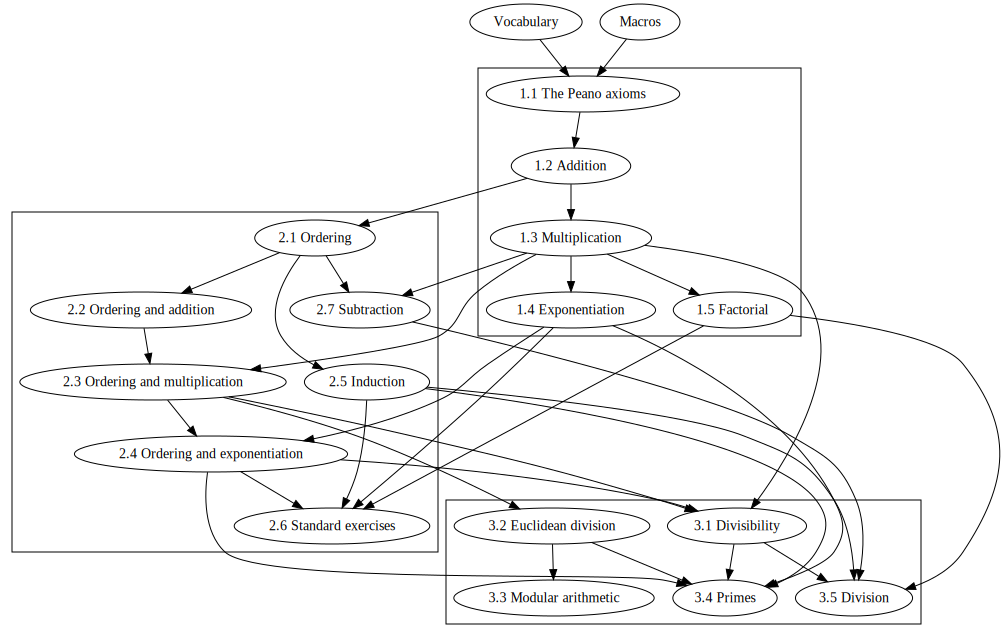
\includegraphics[width=0.9\textwidth]{./dependency-graph/graph.png}}
    \caption*{Interdependencies of the chapters}
  \end{figure}

  \section*{Introduction}

  This is a library providing basic results from undergraduate-level set theory.
  It introduces the notion of transitive classes
  (\cref{chapter:transitive-classes}), defines the notion of ordinal numbers
  (\cref{chapter:ordinals}) and as a special case of the latter introduces the
  set $\omega$ of finite ordinals (\cref{chapter:finite-ordinals}).
  Moreover, this library provides a formalization of the ordinal recursion
  theorem (\cref{chapter:recursion}) which is used to prove Zermelo's
  well-ordering theorem (\cref{chapter:zermelo}), on the basis of which the
  notion of cardinal numbers is introduced (\cref{chapter:cardinals}).
  Furthermore, some results about finite and infinite sets are given
  (\cref{chapter:finite-and-infinite-sets}).

  \paragraph*{Usage.}
  At the very beginning of each chapter you can find the name of its source
  file, e.g. \path{set-theory/sections/01_transitive-classes.ftl.tex} for
  \cref{chapter:transitive-classes}.
  This filename can be used to import the chapter via \Naproche's
  \texttt{readtex} instruction to another ForTheL text, e.g.:
  \begin{center}
    \verb`[readtex \path{set-theory/sections/01_transitive-classes.ftl.tex}]`
  \end{center}

  \paragraph*{Checking times.}
  The checking times for each of the chapters may vary from computer to
  computer, but on mid-range hardware they are likely to be similar to those
  given in table below:

  \begin{center}
    \begin{tabular}{c|c|c}

      & \multicolumn{2}{c}{\textbf{Checking time}}
      \\
      \textbf{Chapter}
      & \textbf{without dependencies}     & \textbf{with dependencies}
      \\ \hline
      \ref{chapter:transitive-classes}
      & 00:20 min                         & 07:00 min
      \\
      \ref{chapter:ordinals}
      & 03:20 min                         & 10:30 min
      \\
      \ref{chapter:finite-ordinals}
      & 01:15 min                         & 11:45 min
      \\
      \ref{chapter:recursion}
      & 04:05 min                         & 14:35 min
      \\
      \ref{chapter:zermelo}
      & 04:45 min                         & 21:40 min
      \\
      \ref{chapter:cardinals}
      & 05:10 min                         & 26:50 min
      \\
      \ref{chapter:finite-and-infinite-sets}
      & 10:50 min                         & 38:55 min
    \end{tabular}
  \end{center}

  \subfile{sections/01_transitive-classes.ftl.tex}
  \subfile{sections/02_ordinals.ftl.tex}
  \subfile{sections/03_finite-ordinals.ftl.tex}
  \subfile{sections/04_recursion.ftl.tex}
  \subfile{sections/05_well-ordering-theorem.ftl.tex}
  \subfile{sections/06_cardinals.ftl.tex}
  \subfile{sections/07_finite-and-infinite-sets.ftl.tex}
\end{document}

\begin{document}
  \begin{imports}
    \begin{forthel}
      %[prove off][check off]

      [readtex \path{libraries/source/set-theory/03_finite-ordinals.ftl.tex}]

      [readtex \path{libraries/source/set-theory/06_cardinals.ftl.tex}]

      %[prove on][check on]
    \end{forthel}
  \end{imports}


  \section{Finite and Infinite Sets}

  \begin{forthel}
    \begin{proposition}\printlabel{SET_THEORY_07_6139396896063488}
      $|\emptyset| = 0$.
    \end{proposition}
  \end{forthel}

  \begin{forthel}
    \begin{proposition}\printlabel{SET_THEORY_07_836893598023680}
      Let $a$ be an object.
      Then $|\set{a}| = 1$.
    \end{proposition}
    \begin{proof}
      Define $f(x) = 0$ for $x \in \set{a}$.
      Then $f$ is a map from $\set{a}$ to $1$.
      $f$ is injective and surjective onto $1$.
      Hence $f$ is a bijection between $\set{a}$ and $1$.
      Consequently $\set{a}$ and $1$ are equinumerous.
      Thus $|\set{a}| = |1| = 1$.
    \end{proof}
  \end{forthel}

  \begin{forthel}
    \begin{proposition}\printlabel{SET_THEORY_07_5465279026954240}
      Let $a, b$ be distinct objects.
      Then $|\set{a,b}| = 2$.
    \end{proposition}
    \begin{proof}
      Define \[ f(x) =
        \begin{cases}
          0 & x = a
          \\
          1 & x = b
        \end{cases} \]
      for $x \in \set{a,b}$.
      Then $f$ is a map from $\set{a,b}$ to $2$.
      $f$ is injective and surjective onto $2$.
      Hence $f$ is a bijection between $\set{a,b}$ and $2$.
      Consequently $\set{a,b}$ and $2$ are equinumerous.
      Thus $|\set{a,b}| = |2| = 2$.
    \end{proof}
  \end{forthel}

  \begin{forthel}
    \begin{theorem}\printlabel{SET_THEORY_07_2948332552978432}
      Let $n \in \omega$.
      Then $|n| = n$.
    \end{theorem}
    \begin{proof}
      Define $\Phi = \{ n' \in \omega \mid |n'| = n' \}$.

      (1) $0 \in \Phi$.
      Indeed $|0| = |\emptyset| = 0$.

      (2) For all $n' \in \Phi$ we have $\succ(n') \in \Phi$. \\
      Proof.
        Let $n' \in \Phi$.
        Then $|n'| = n'$.
        We have $|\succ(n')| \leq \succ(n')$.

        Let us show that $\succ(n') \leq |\succ(n')|$.
          Assume the contrary.
          Then $|\succ(n')| < \succ(n')$.
          Take a bijection $f$ between $|\succ(n')|$ and $\succ(n')$.
          $|\succ(n')|$ is nonzero.
          Hence we can take a $m \in \omega$ such that $|\succ(n')| =
          \succ(m)$.
          Then $f^{-1}(n') \leq m$.

          We can show that $f^{-1}(n') < m$.
            Assume the contrary.
            Then $f^{-1}(n') = m$.
            $f \restriction m$ is a bijection between $m$ and $f[m]$ (by
            \cref{FOUNDATIONS_08_647446231252992}).
            Indeed $f$ is an injective map from $|\succ(n')|$ to $\succ(n')$ and
            $m \subseteq |\succ(n')|$.
            We have $f[m] \subseteq n'$ and $n' \subseteq f[m]$.
            Hence $f[m] = n'$.
            Thus $f \restriction m$ is a bijection between $m$ and $n'$.
            Therefore $n'
              = |n'|
              \leq m
              < |\succ(n')|
              < \succ(n')$.
            Consequently $m = n'$.
            Then we have $\succ(n') = |\succ(n')| < \succ(n')$.
            Contradiction.
          End.

          Define \[ g(i) =
            \begin{cases}
              f(i)  & : i \neq f^{-1}(n')
              \\
              f(m)  & : i = f^{-1}(n')
            \end{cases} \]
          for $i \in m$.

          $g$ is a map from $m$ to $n'$.
          Indeed we can show that $g(i) \in n'$ for each $i \in m$. \\
          Proof.
            Let $i \in m$.

            Case $i \neq f^{-1}(n')$.
              Then $g(i) = f(i) \in \succ(n')$.
              If $g(i) = n'$ then $f(i) = n' = f(f^{-1}(n'))$.
              Hence if $g(i) = n'$ then $i = f^{-1}(n')$.
              Thus $g(i) \neq n'$.
              Therefore $g(i) \in n'$.
            End.

            Case $i = f^{-1}(n')$.
              Then $g(i)
                = f(m)
                \neq f(f^{-1}(n'))
                = n'$.
              Hence $g(i) \in n'$.
            End.
          Qed.

          $g$ is surjective onto $n'$.
          Indeed we can show that for all $k \in n'$ there exists a $l \in m$
          such that $k = g(l)$. \\
          Proof.
            Let $k \in n'$.
            Then $f^{-1}(k) \neq f^{-1}(n')$.

            Case $f^{-1}(k) = m$.
              Then $k
                = f(f^{-1}(k))
                = f(m)
                = g(f^{-1}(n'))$.
            End.

            Case $f^{-1}(k) \neq m$.
              Then $f^{-1}(k) \in m$.
              Indeed $f^{-1}(k) \in |\succ(n')| = \succ(m) = m \cup \set{m}$.
              Hence $k
                = f(f^{-1}(k))
                = g(f^{-1}(k))$.
            End.
          Qed.

          $g$ is injective.
          Indeed we can show that for all $i, j \in m$ if $i \neq j$ then
          $g(i) \neq g(j)$. \\
          Proof.
            Let $i, j \in m$.
            Assume $i \neq j$.

            Case $i, j \neq f^{-1}(n')$.
              Then $g(i)
                = f(i)
                \neq f(j)
                = g(j)$.
            End.

            Case $i = f^{-1}(n')$.
              Then $j \neq f^{-1}(n')$.
              Hence $g(i)
                = g(f^{-1}(n'))
                = f(m)
                \neq f(j)
                = g(j)$.
              Indeed $m \neq j$.
            End.

            Case $j = f^{-1}(n')$.
              Then $i \neq f^{-1}(n')$.
              Hence $g(i)
                = f(i)
                \neq f(m)
                = g(f^{-1}(n'))
                = g(j)$.
              Indeed $i \neq m$.
            End.
          Qed.
        End.
      End.

      Thus $\omega \subseteq \Phi$ (by \cref{SET_THEORY_03_344585425387520}).
      Consequently $n \in \Phi$.
      Therefore $|n| = n$.
    \end{proof}
  \end{forthel}

  \begin{forthel}
    \begin{corollary}\printlabel{SET_THEORY_07_7061392098066432}
      Every element of $\omega$ is a cardinal.
    \end{corollary}
  \end{forthel}

  \begin{forthel}
    \begin{proposition}\printlabel{SET_THEORY_07_4952029518626816}
      $|\omega| = \omega$.
    \end{proposition}
    \begin{proof}
      We have $|\omega| \leq \omega$.

      Let us show that $|\omega|$ is not less than $\omega$.
        Assume the contrary.
        Then $|\omega| \in \omega$.
        Take $n = |\omega|$ and a bijection $f$ between $n$ and $\omega$.

        Define \[ g(k) =
          \begin{cases}
            \succ(f(k)) & : k < n
            \\
            0           & : k = n
          \end{cases} \]
        for $k \in \succ(n)$.
        Then $g$ is a map from $\succ(n)$ to $\omega$.

        $g$ is injective.
        Indeed we can show that for all $k, k' \in \succ(n)$ if $k \neq k'$
        then $g(k) \neq g(k')$. \\
        Proof.
          Let $k, k' \in \succ(n)$.
          Assume $k \neq k'$.

          Case $k, k' < n$.
            Then $f(k) \neq f(k')$.
            Hence $\succ(f(k)) \neq \succ(f(k'))$.
            Thus $g(k) \neq g(k')$.
          End.

          Case $k < n$ and $k' = n$.
            We have $\succ(f(k)) \neq 0$.
            Hence $g(k) \neq g(k')$.
          End.

          Case $k = n$ and $k' < n$.
            We have $\succ(f(k')) \neq 0$.
            Hence $g(k) \neq g(k')$.
          End.
        Qed.

        $g$ is surjective onto $\omega$.
        Indeed we can show that for any $m \in \omega$ there exists a
        $k \in \succ(n)$ such that $m = g(k)$. \\
        Proof.
          Let $m \in \omega$.
          Then $f^{-1}(m) \in n$.

          Case $m = 0$.
            Then $m = g(n)$.
          End.

          Case $m \neq 0$.
            Take $m' \in \omega$ such that $m = \succ(m')$.
            Then $m
              = \succ(m')
              = \succ(f(f^{-1}(m')))
              = g(f^{-1}(m'))$.
            Indeed $f^{-1}(m') < n$.
          End.
        End.

        Hence $g$ is a bijection between $\succ(n)$ and $\omega$.
        Then we have $|n| = |\succ(n)|$.
        Thus $n = \succ(n)$.
      End.
    \end{proof}
  \end{forthel}

  \begin{forthel}
    \begin{corollary}\printlabel{SET_THEORY_07_2717623053713408}
      $\omega$ is a cardinal.
    \end{corollary}
  \end{forthel}

  \begin{forthel}
    \begin{definition}\printlabel{SET_THEORY_07_5346658235711488}
      Let $x$ be a set.
      $x$ is finite iff $|x| < \omega$.
    \end{definition}
  \end{forthel}

  \begin{forthel}
    \begin{definition}\printlabel{SET_THEORY_07_8295412068777984}
      Let $x$ be a set.
      $x$ is infinite iff $x$ is not finite.
    \end{definition}
  \end{forthel}

  \begin{forthel}
    \begin{definition}\printlabel{SET_THEORY_07_8808604616359936}
      Let $x$ be a set.
      $x$ is countable iff $|x| \leq \omega$.
    \end{definition}
  \end{forthel}

  \begin{forthel}
    \begin{definition}\printlabel{SET_THEORY_07_2935263915409408}
      Let $x$ be a set.
      $x$ is uncountable iff $x$ is not countable.
    \end{definition}
  \end{forthel}

  \begin{forthel}
    \begin{definition}\printlabel{SET_THEORY_07_5679866426949632}
      Let $x$ be a set.
      $x$ is countably infinite iff $|x| = \omega$.
    \end{definition}
  \end{forthel}

  \begin{forthel}
    \begin{proposition}\printlabel{SET_THEORY_07_3806229474312192}
      Let $x$ be a set.
      Then $x$ is finite iff $|x| = n$ for some $n \in \omega$.
    \end{proposition}
  \end{forthel}

  \begin{forthel}
    \begin{proposition}\printlabel{SET_THEORY_07_3174577070931968}
      Let $x$ be a set.
      Then $x$ is infinite iff $|x| \geq \omega$.
    \end{proposition}
    \begin{proof}
      $|x| \geq \omega$ iff $|x| \nless \omega$.
    \end{proof}
  \end{forthel}

  \begin{forthel}
    \begin{proposition}\printlabel{SET_THEORY_07_4281623468048384}
      Let $x$ be a set.
      Then $x$ is uncountable iff $|x| > \omega$.
    \end{proposition}
  \end{forthel}

  \begin{forthel}
    \begin{definition}\printlabel{SET_THEORY_07_4231078585827328}
      $\Card$ is the collection of all infinite cardinals.
    \end{definition}
  \end{forthel}

  \begin{forthel}
    \begin{proposition}\printlabel{SET_THEORY_07_4285360123150336}
      $\Card$ is a proper class.
    \end{proposition}
    \begin{proof}
      Suppose that $\Card$ is a set.
      Then $\bigcup \Card$ is a set.

      Let us show that $\bigcup \Card$ contains every ordinal.
        Let $\alpha$ be an ordinal.
        Choose an infinite ordinal $\beta$ such that $\beta \geq \alpha$.
        Choose a cardinal $\kappa$ greater than $\beta$.
        Then $\alpha \in \kappa \in \Card$.
        Hence $\alpha \in \bigcup \Card$.
      End.

      Therefore $\Ord \subseteq \bigcup \Card$.
      Thus $\Ord$ is a set.
      Contradiction.
    \end{proof}
  \end{forthel}

  \begin{forthel}
    \begin{proposition}\printlabel{SET_THEORY_07_8189062544359424}
      Let $\alpha$ be an infinite ordinal.
      Then $|\succ(\alpha)| = |\alpha|$.
    \end{proposition}
    \begin{proof}
      For any $\beta \in \succ(\alpha)$ we have
      $\beta < \omega$ or $\omega \leq \beta < \alpha$ or $\beta = \alpha$.
      Define \[ f(\beta) =
        \begin{cases}
          \succ(\beta)  & : \beta < \omega
          \\
          \beta         & : \omega \leq \beta < \alpha
          \\
          0             & : \beta = \alpha
        \end{cases} \]
      for $\beta \in \succ(\alpha)$.

      Then $f$ is a map from $\succ(\alpha)$ to $\alpha$.
      Indeed we can show that $f(\beta) \in \alpha$ for all
      $\beta \in \succ(\alpha)$. \\
      Proof.
        Let $\beta \in \succ(\alpha)$.

        Case $\beta < \omega$.
          Then $f(\beta)
            = \succ(\beta)
            < \omega
            \leq \alpha$.
        End.

        Case $\omega \leq \beta < \alpha$.
          Then $f(\beta)
            = \beta
            < \alpha$.
        End.

        Case $\beta = \alpha$.
          Then $f(\beta)
            = 0
            < \alpha$.
        End.
      Qed.

      $f$ is surjective onto $\alpha$.
      Indeed we can show that for any $\beta \in \alpha$ there exists a
      $\gamma \in \succ(\alpha)$ such that $\beta = f(\gamma)$. \\
      Proof.
        Let $\beta \in \alpha$.
        Then $\beta = 0$ or $0 < \beta < \omega$ or $\beta \geq \omega$.

        Case $\beta = 0$.
          Then $\beta = f(\alpha)$.
        End.

        Case $0 < \beta < \omega$.
          Take an ordinal $\beta'$ such that $\beta = \succ(\beta')$.
          Then $\beta' < \omega$.
          Hence $\beta = f(\beta')$.
        End.

        Case $\beta \geq \omega$.
          Then $\beta = f(\beta)$.
        End.
      Qed.

      $f$ is injective.
      Indeed we can show that for all $\beta, \gamma \in \succ(\alpha)$ if
      $\beta \neq \gamma$ then $f(\beta) \neq f(\gamma)$. \\
      Proof.
        Let $\beta, \gamma \in \succ(\alpha)$.
        Assume $\beta \neq \gamma$.

        Case $\beta < \omega$.
          If $\gamma = \alpha$ then
          $f(\beta)
            = \succ(\beta)
            \neq 0
            = f(\gamma)$.
          If $\omega \leq \gamma < \alpha$ then
          $f(\beta)
            = \succ(\beta)
            < \omega
            \leq \gamma
            = f(\gamma)$.
        End.

        Case $\omega \leq \beta < \alpha$.
          If $\gamma = \alpha$ then
          $f(\beta)
            = \beta
            \geq \omega
            > 0
            = f(\gamma)$.
          If $\gamma < \omega$ then
          $f(\beta)
            = \beta
            \geq \omega
            > \succ(\gamma)
            = f(\gamma)$.
        End.

        Case $\beta = \alpha$.
          If $\gamma < \omega$ then
          $f(\beta)
            = 0
            \neq \succ(\gamma)
            = f(\gamma)$.
          If $\omega \leq \gamma < \alpha$ then
          $f(\beta)
            = 0
            < \omega
            \leq \gamma
            = f(\gamma)$.
        End.
      Qed.

      Hence $f$ is a bijection between $\succ(\alpha)$ and $\alpha$.
      Therefore $\succ(\alpha)$ and $\alpha$ are equinumerous.
      Consequently $|\succ(\alpha)| = |\alpha|$.
    \end{proof}
  \end{forthel}

  \begin{forthel}
    \begin{proposition}\printlabel{SET_THEORY_07_8700732632989696}
      Every infinite cardinal is a limit ordinal.
    \end{proposition}
    \begin{proof}
      Let $\kappa$ be an infinite cardinal.
      Suppose that $\kappa$ is not a limit ordinal.
      $\kappa \neq 0$.
      Hence $\kappa$ is a successor ordinal.
      Thus we can take an ordinal $\alpha$ such that $\kappa = \succ(\alpha)$.
      We have $\alpha > \kappa \geq \omega$.
      Hence $|\succ(\alpha)| = |\alpha|$.
      Thus $\alpha < |\kappa|$ and $\kappa$ is equinumerous to $\kappa$.
      Contradiction.
    \end{proof}
  \end{forthel}
\end{document}
